\section{Dynamic Simulation of HSA Robots}\label{sec:hsamodel:hsa_robot_simulation}
We introduce a new concept to enable the simulation of \gls{HSA} robots with the discretized Cosserat rod theory, which is used by many of the SoA simulators of soft continuum robots~\citep{naughton2021elastica, mathew2022sorosim}.
While we provide an implementation of the proposed concept as a plugin to Elastica~\citep{naughton2021elastica}, the same strategy could be used to adapt other simulators such as SoRoSim~\citep{mathew2022sorosim} to \gls{HSA} robots.
% The proposed mechanism couples the rest length of the rods with their twist strains to mirror the auxetic trajectory and modifies the stiffness of the rod as a function to the twist strain to match the known mechanical characteristics of \glspl{HSA}. %~\citep{good2022expanding}.
% We provide an implementation of this strategy through a plugin for the Elastica simulator~\citep{naughton2021elastica}.
% Our simulator is based on a discretized version of the Cosserat rod theory~\citep{renda2018discrete, gazzola2018forward, naughton2021elastica, mathew2022sorosim} and allows the user to simulate the behaviour of a system consisting of $n_\mathrm{HSA}$ rods, each with a handedness $h_j \in \{-1, 1 \}$, and a rigid cylindrical platform constraining all of the \glspl{HSA} at their tips.
%
We give some background on the \gls{DCM} in Section~\ref{sub:hsamodel:hsa_robot_simulation:discretized_cosserat_rod_model}. Then, in \ref{sub:hsamodel:hsa_robot_simulation:auxetic_trajectory}, we propose a mechanism to infuse the auxetic trajectory for a \gls{HSA} into the \gls{DCM} framework. Subsequently, we verify the steady-state behavior of an \gls{HSA} against the mechanical characteristics in \ref{sub:hsamodel:hsa_robot_simulation:verification_good}. Next, we lay out in \ref{sub:hsamodel:hsa_robot_simulation:hsa_robots} the necessary boundary conditions of the \glspl{HSA} and describe the joint mechanism connecting the platform with the rods. Finally, we explain in Section~\ref{sub:hsamodel:hsa_robot_simulation:motion_primitives} how we were able to reproduce in simulation the main motion primitives of \gls{HSA} robots.

\subsection{Background: Discretized Cosserat Rod Model}\label{sub:hsamodel:hsa_robot_simulation:discretized_cosserat_rod_model}
This subsection will introduce the governing equations of the \gls{DCM} following the work by \citet{gazzola2018forward}.
According to the Cosserat rod theory, a slender rod's shape can be purely described by the line along its backbone. % The coordinate $s \in [0,L] \in \mathbb{R}$ can then be used to define a point along the backbone. % arc-length coordinate
The backbone curve is divided into a discrete set of nodes with position $r_i(t) \in \mathbb{R}^3 \: \forall \: i \in \{1,\dots,n_\mathrm{v}+1\}$ and $n_\mathrm{v}$ links of orientation $Q_i(t) \in \mathbb{R}^{3 \times 3}$.
Differentiating the position and orientation with respect to time gives the translational and angular velocities $v_i = \frac{\partial r_i}{\partial t} \in \mathbb{R}^3$ and $\omega_{\mathcal{L}}^i \in \mathbb{R}^3$.
% The $\mathcal{L}$ subscript denotes that the quantity lives in the body-convected frame, while all other variables are described in the inertial frame.
Each node has a mass of $m_i$, and the rigid links are modeled to have a second mass moment of inertia $J_i$.
When a rod of unstretched length $\hat{L}$ is at rest, each link has a length of $\hat{l}_i$ and connects two consecutive vertices. 
The circumflex accent will denote quantities in the rest configuration of the rod.
When the rod is in a deformed state, $l$ describes the current edge length and
% In contrast to the Kirchoff-Love theory, which does not allow for shear and extension to occur, the Cosserat rod theory accounts for all six deformation modes. 
the shear and axial strains are considered in the vector $\sigma = \begin{pmatrix} \sigma_x & \sigma_y & \sigma_z \end{pmatrix}^\top$. The curvature vector $\kappa_{\mathcal{L}} = \begin{pmatrix} \kappa_x & \kappa_y & \kappa_z \end{pmatrix}^\top$ captures the bending and twist strains.
All strains are defined with respect to the rest length of the link $\hat{l}_i$, and the dilation factor $e_i = \frac{l_i}{\hat{l}_i}$ denotes the deviation from that rest length.
The shear and stretch stiffness is specified through the diagonal matrix $S = \mathrm{diag}(E I_{xx}, E I_{yy}, G I_{zz}) \in \mathbb{R}^{3 \times 3}$, where $E$, $G$ are the elastic and shear modulus respectively, and $I \in \mathbb{R}^{3 \times 3}$ is the second area moment of inertia. Analogue, the bending and twist rigidity is stored in $B = \mathrm{diag}(B_x, B_y, B_z) \in \mathbb{R}^{3 \times 3}$.
For conciseness, we include only the equation for the translational accelerations below. We refer the interested reader to \citep{gazzola2018forward} for the equation on rotational accelerations and more complementary details about the \gls{DCM}.
% The translational and rotational accelerations are then given as part of the governing equations as
\begin{align}
    m_i \frac{\partial v_i}{\partial t} =& \Delta^h \left ( \frac{Q_i^\top \hat{S}_i \sigma^i_{\mathcal{L}}}{e_i} \right ) + F_i, \quad i\in \{1,\dots,n_\mathrm{v}+1\},
    %\frac{\hat{J}_i}{e_i} \frac{\partial\omega_{\mathcal{L}}^i}{\partial t} =& \Delta^h \left ( \frac{\hat{B}_i \hat{\kappa}_{\mathcal{L}}^i}{\epsilon^3_i} \right ) + \mathcal{A}^h \left ( \frac{\hat{\kappa}_{\mathcal{L}}^i \times \hat{B}_i \hat{\kappa}^i_{\mathcal{L}}}{\epsilon^3_i} \right )\notag\\
    %&+ (Q_i t_i \times \hat{S}_i \sigma_{\mathcal{L}}^i)\hat{l}_i + \left ( \hat{J}_i \frac{\omega^i_{\mathcal{L}}}{e_i} \right ) \times \ \omega_{\mathcal{L}}^i\notag\\
    % &+\frac{\hat{J}_i \omega^i_{\mathcal{L}}}{e_i^2} \frac{\partial e_i}{\partial t} + \tau_{\mathcal{L}}^i, \quad i=[1,n_\mathrm{v}],
\end{align}
where $F_i \in \mathbb{R}^3$ is the external force acting on the $i$th vertex.
Several quantities are expressed in the Voronoi domain $\mathcal{D}$, in which the length of the region $\mathcal{D}_i$ can be computed as $\mathcal{D}_i = \frac{l_{i+1} + l_i}{2}, i \in [1,n_\mathrm{v}-1]$. Examples are the % Voronoi dilation $\epsilon_i$, 
the Voronoi curvature $\hat{\kappa}_{\mathcal{L}}^i$ over the interior vertices, and the bend twist stiffness matrix $\hat{B}_i$.
$\Delta^h : \{\mathbb{R}^3 \}_N \rightarrow \{ \mathbb{R}^3 \}_{N+1}$ is used as the discrete difference operator.
% where $F_i \in \mathbb{R}^3$ and $\tau^i_{\mathcal{L}} \in \mathbb{R}^3$ are the external force and couple acting on the $i$th vertex and link respectively.
% Several quantities were expressed in the Voronoi domain $\mathcal{D}$, in which the length of the region $\mathcal{D}_i$ can be computed as $\mathcal{D}_i = \frac{l_{i+1} + l_i}{2}, i \in [1,n_\mathrm{v}-1]$. Examples are the Voronoi dilation $\epsilon_i$, the Voronoi curvature $\hat{\kappa}_{\mathcal{L}}^i$ over the interior vertices, and the bend twist stiffness matrix $\hat{B}_i$.
% $\Delta^h : \{\mathbb{R}^3 \}_N \rightarrow \{ \mathbb{R}^3 \}_{N+1}$ is used as the discrete difference operator and $\mathcal{A}^h : \{\mathbb{R}^3 \}_N \rightarrow \{ \mathbb{R}^3 \}_{N+1}$ averages over $\mathcal{D}$ to get the corresponding values in the node domain.

\subsection{Auxetic Trajectory}\label{sub:hsamodel:hsa_robot_simulation:auxetic_trajectory}
% We implement several modifications and extension to the Elastica simulator~\citep{gazzola2018forward} to allow for realistic simulation of \glspl{HSA}.
We propose several adjustments to the standard definition of the \gls{DCM} to allow for realistic simulation of \glspl{HSA}.
The main assumption behind the proposed concept is that twist strains agreeing with the handedness of the rod will modify the internal angle between the auxetic pattern cells and, with that, also change the system characteristics such as spring constant, blocked force, etc.

Most importantly, we introduce a distinction between the printed, initial length of the \gls{HSA} $\bar{L}$ and the rest length of the rod $\hat{L}$. 
This allows us to mirror the auxetic trajectory, as the minimum energy length is increased with applied twist angles / strains~\citep{good2022expanding}.
Similar to the \textsc{hat} accent, which denotes rest quantities, the \textsc{bar} accent will point out quantities of the \gls{HSA} in the initial / printed state.
%As an example, when the twist strain $\kappa_{\mathcal{L},z}$ is zero, $\bar{L} = \hat{L}$. However when twist strains are present, 
We propose to linearly scale the edge rest length $\hat{l}_i$ with the twist strain $\kappa_{\mathcal{L},z}^i$:
\begin{align}
    \hat{l}_i &= (1 + \varepsilon_i) \, \bar{l} \quad i\in \{1,\dots,n_\mathrm{v}+1\},\\
  \varepsilon_i &= \max \left (\min \left (h \: C_{\varepsilon} \, \mathcal{A}^h(\kappa_{\mathcal{L},z}^i),\varepsilon_\mathrm{max} \right ), \varepsilon_\mathrm{min} \right ).
\end{align}
In this expression, the twist strain $\kappa_{\mathcal{L},z}^i$ is elevated from the Voronoi to the vertex domain with the averaging operator $\mathcal{A}^h : \{\mathbb{R}^3 \}_N \rightarrow \{ \mathbb{R}^3 \}_{N+1}$. $h \in \{ -1, 1 \}$ is the handedness of the rod. Right is defined as the positive, and left as the negative handedness.
$C_{\varepsilon}$ is the extension factor, which needs to be tuned with respect to the chosen auxetic pattern.
The minimum and maximum extension $\varepsilon_\mathrm{min}$, $\varepsilon_\mathrm{max}$ are the limits of the auxetic trajectory and depend on the \gls{HSA} type: for example, closed \glspl{HSA} can only exhibit positive elongations~\citep{good2022expanding}. % Contrarily, semi-open \glspl{HSA} can both contract and elongate~\citep{good2022expanding}.
After the rest length is adjusted, the axial stiffness of the rod will guide the current edge length $l_i$ towards the (target) edge rest length. % $\hat{l}_i \neq \bar{l}_i$
% This strategy allows us to keep the axial deformability in tact, while adjusting the length of the rod according to the auxetic trajectory.
Furthermore, we recall the definition of bend/twist strains: $\kappa_{\mathcal{L}}^i = \frac{\log(Q_{i+1} \: Q_i^\top)}{\hat{\mathcal{D}}_i}$. 
% As the rest length is changed while traversing the auxetic trajectory, the Voronoi rest length $\hat{\mathcal{D}}_i$ and therefore the twist strain $\kappa_{\mathcal{L}}^i$ would change as well. 
To keep the twist strain constant across the entire auxetic trajectory, we define the twist strain with respect to the initial Voronoi length $\bar{\mathcal{D}}_i = \frac{\bar{l}_{i+1} - \bar{l}_i}{2}$:
\begin{equation}
    \kappa_{\mathcal{L},z}^i = \frac{\log(Q_{i+1} \: Q_i^\top)}{\bar{\mathcal{D}}_i}, \quad i\in \{1,\dots,n_\mathrm{v}+1\}
\end{equation}

\begin{table}[hbt]
\centering
\caption{Parameters of simulated HSA rods in Section~\ref{sub:hsamodel:hsa_robot_simulation:verification_good} for various number of HSA row tilings $n_\mathrm{rows}$. Row tilings represent the number of vertically stacked unit cells~\citep{good2022expanding}. The rest length $\hat{L}$ and the elastic modulus $E$ are linear functions of the twist strain $\kappa_z$. $B_z$ represents the twist rigidity.}
\begin{tabular}{c ccc}\toprule
$n_\mathrm{rows}$ & $\hat{L} \, [\si{mm}]$ & $E \, [\si{kPa}]$ & $B_z \, [\si{Nm^2 \per rad}]$\\
\midrule
$4$ & $75 \, (1 + 3.04 \: \kappa_z)$ & $576.9 + 36.1 \: \kappa_z$ & $0.00375$\\
$6$ & $89 \, (1 + 3.50 \: \kappa_z)$ & $309.3 + 13.1 \: \kappa_z$ & $0.00213$\\
$8$ & $100 \, (1 + 3.77 \: \kappa_z)$ & $203.5 + 10.6 \: \kappa_z$ & $0.00183$\\
$10$ & $112 \, (1 + 3.64 \: \kappa_z)$ & $197.6 + 7.5 \: \kappa_z$ & $0.00167$\\
$12$ & $124 \, (1 + 3.53 \: \kappa_z)$ & $197.6 + 2.4 \: \kappa_z$ & $0.00124$\\
\bottomrule
\end{tabular}
\label{tab:hsamodel:hsa_rod_parameters_sim_verification}
\end{table}

Finally, recent work by \citet{good2022expanding} has shown that \glspl{HSA} exhibits special mechanical characteristics, such as the spring constant increasing with the twist angle. Therefore, we allow the shear/stretch and bend / twist rigidity matrices $S$ and $B$ to be modified dynamically during the simulation with the twist strain. For example, the axial stiffness of a closed \gls{HSA} can be modeled as a linear function of the twist strain~\citep{good2022expanding}
\begin{equation}
    \hat{S}_{z}^i = \Bar{S}_{z}^i + C_{S_z} \mathcal{A}^h(\kappa_{\mathcal{L},z}^i),
\end{equation}
where $C_{S_z}$ is a tunable constant.

\subsection{Verification of HSA Rod Steady-State Behaviour}\label{sub:hsamodel:hsa_robot_simulation:verification_good}
We verify that our simulator can represent the steady-state behavior of a real \gls{HSA} by re-producing the characterization results for closed \glspl{HSA} by \citet{good2022expanding}.
More specifically, we let the simulator converge to a steady state and then identify several mechanical properties such as blocked force ($F_\mathrm{b}$), minimum energy length, holding torque ($\tau_\mathrm{h}$), and the spring constant ($k$).
Following the reporting in \citep{good2022expanding}, we tune the parameters of our simulation to match the behavior of closed Carbon FPU50 \glspl{HSA} with \SI{19}{mm} outside diameter, \SI{2}{mm} wall thickness, as good as possible. We report the chosen simulation parameters in Table~\ref{tab:hsamodel:hsa_rod_parameters_sim_verification}. 
The \gls{HSA} rod is modelled to consist of $n_\mathrm{v} = 10$ nodes and $9$ links with a material density of $\rho = \SI{1050}{kg \per m^3}$. For all simulations, the proximal end of the rod is constrained, and only rotations around the z-axis are allowed to mirror the actuation with electric motors. Furthermore, twisting is constrained at the distal end, which allows twist strains to build up in the rod. Otherwise, the distal end is unconstrained.

\begin{figure*}[hbt]
    \centering
    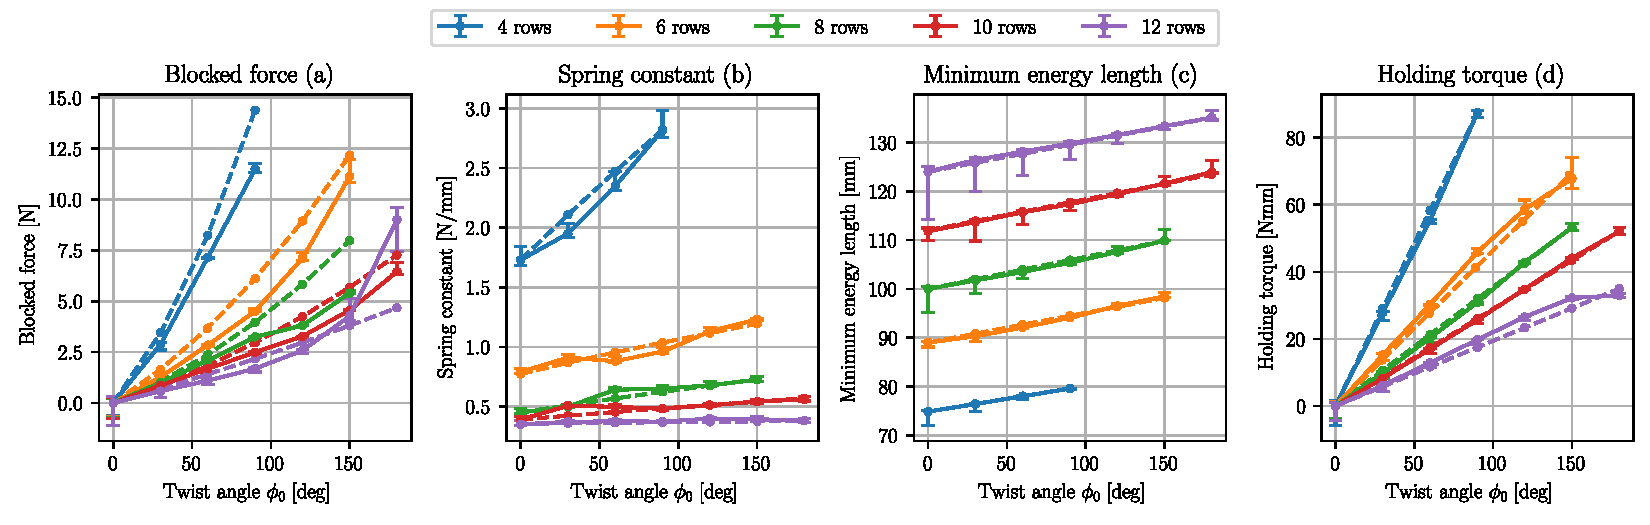
\includegraphics[width=\textwidth]{hsamodel/figures/simulation/closed_hsa_rods_verification_v2.pdf}
    \caption{Results for verification of steady-state behavior of the proposed simulator: the solid lines represent the mechanical characteristics obtained for closed \gls{HSA} rods by \citet{good2022expanding} with corresponding error bars. The dashed lines correspond to the same characteristics obtained with our simulator. The simulation parameters are separately tuned for HSAs with a variety of row tilings. When an HSA contains a higher number of row tiling, it will allow for larger elongations while simultaneously trading off the spring constant~\citep{good2022expanding}.}
    \label{fig:hsamodel:closed_hsa_properties_good_et_al}
\end{figure*}

Next, we will go into more detail about each mechanical characteristic.
\textbf{Holding torque:} We apply a given torsional torque $\tau_\mathrm{h}$ at the proximal end of the \gls{HSA} and then record the twist angle of the base $\phi_0$ at steady-state.
\textbf{Minimum energy length:} The proximal end of the \gls{HSA} is rotated to a given twist angle $\phi_0$. The minimum energy length is then identified as the steady-state length of the \gls{HSA}.
\textbf{Spring constant:} For a given twist angle $\phi_0$ with the \gls{HSA} at rest, the spring constant is identified by applying a small pulling force to the distal end and then measuring the displacement of the tip at steady-state.
\textbf{Blocked force:} Different from the other simulations, the distal end is constrained at its initial position to prevent the rod from extending. The blocked force $F_\mathrm{b}$ is identified by evaluating the internal axial force for a given twist angle.
% We refer the interested reader to the paper by \citet{good2022expanding} for more details on the exact identification procedure of each characteristics.

% Next, we will go into more detail about the identification procedure for each property.
% \subsubsection{Holding torque}
% A given torsional torque $\tau_\mathrm{h}$ is applied to the proximal end of the \gls{HSA} rod while the dynamic behaviour of the rod is simulated for \SI{10}{s} and the last twist angle $\phi_0$ at the proximal end is recorded. This procedure is repeated for a range of torsional torques and the twist angles are plotted against their corresponding holding torques in Fig.~\ref{fig:hsamodel:closed_hsa_properties_good_et_al}(a).

% \subsubsection{Minimum energy length}
% The boundary condition at the proximal end is used to apply a given twist angle. The system is simulated for \SI{10}{s}. The final length of the rod is plotted against the twist angle in Fig.~\ref{fig:hsamodel:closed_hsa_properties_good_et_al}(b).

% \subsubsection{Spring constant}
% Again, a given twist angle is applied to the proximal end and the system is given \SI{10}{s} to converge to steady-state at the respective minimum energy length. Then, we apply a small force $F_z$ of magnitude \SI{1}{N} in z-direction to the tip of the rod and wait another \SI{10}{s} for the rod to be elongated. Subsequently, the displacement of the tip $\delta z$ with respect to the minimum energy length is computed and the spring constant is computed as $k = \frac{F_z}{\delta z}$.

% \subsubsection{Blocked force}
% Differently from the other simulations, the z-position of the distal end is constrained to remain fixed, which prevents the rod from extending. Now, a twist angle is applied at the base and the internal axial force at the tip is plotted against the twist angle.

The results show that the proposed simulator can accurately represent the steady-state behavior of the \glspl{HSA} with the simulated characteristics mostly staying within the stated error range of the experimental measurements by \citet{good2022expanding}. The only exception is Fig.~\ref{fig:hsamodel:closed_hsa_properties_good_et_al}(a), in which the simulation is overestimating the blocked force $F_\mathrm{b}$. This points to the fact that this linear approximation of the auxetic trajectory is only accurate in a limited range of the motion range of the closed \glspl{HSA}. Further research is necessary to come up with auxetic trajectory models for semi-closed and open \glspl{HSA}.

\subsection{Simulating HSA Robots: Boundary Conditions and Joints}\label{sub:hsamodel:hsa_robot_simulation:hsa_robots}
%In the previous subsections, we have devised a strategy for simulating \gls{HSA} rods and have successfully verified the steady-state behaviour of such single \glspl{HSA}. Now, 
%
We discuss here how to combine a platform and multiple \glspl{HSA} to form a \gls{HSA} robot.  Assume to have $n_\mathrm{HSA}$ rods equally distributed along a circle of radius $R_\mathrm{cHSA}$ in the x-y plane with the rods pointing towards the positive z-direction in a straight configuration.
%
We need boundary conditions for the proximal ends of the rods to generate the parallel structure. The positions of the proximal nodes are constrained to remain at their initial position $\bar{r}_{0}$.
% $\bar{r}_{0} = \begin{pmatrix} \cos(\varphi) R_\mathrm{cHSA} & \sin(\varphi)R_\mathrm{cHSA} & 0 \end{pmatrix}^\top$, where $\varphi$ is the azimuth angle. 
For the same purpose, the translational rates, e.g., $v_0$, are set to zero at each time step. 

In our plug-in to Elastica, we provide the user with two options for actuating the \glspl{HSA}. (a) The orientation of the proximal link $Q_{0}$ is moved to a desired orientation $Q_{0}^\mathrm{d}$. In this case, the twist angle $\phi_0^\mathrm{d}$ of the proximal end is controlled. Again, the rotational rates $\omega_0$ are set to zero. 
(b) Twist torques $\tau_{0,z}$ are applied to the proximal link of the \gls{HSA}. The two remaining rotational \glspl{DOF} (rolling and pitching) of the proximal link are constrained by setting their rotational rates $\omega_{0,x}$ and $\omega_{0,y}$ to zero.

Additionally, rigid joints between the rods and the platform are necessary. These are achieved by simulating a spring-damper system between the distal end of each \gls{HSA} and the platform. For the translations, we compute the contact force $F_\mathrm{c}$ as 
\begin{equation}
    F_\mathrm{c} = k_F \, (r_\mathrm{p}^j - r_{n_\mathrm{v}+1}) + \nu_F \, (v_\mathrm{p}^j - v_{n_\mathrm{v}+1}),
\end{equation}
where $k_F$ is the translational joint stiffness, and $\nu_F$ the translational damping coefficient. While $r_{n_\mathrm{v}+1}$, and $v_{n_\mathrm{v}+1}$ are the position and the velocity of the distal node of the rod, respectively, $r_\mathrm{p}^j$ and $v_{n_\mathrm{v}+1}^j)$ are the position and velocity of the attachment point of the same rod (e.g. the $j$th rod) on the platform. We determine the position and velocity of this attachment point using rigid body kinematics with regard to the \gls{COM} of the platform. The contact force $F_\mathrm{c}$ is applied with an opposite sign to the distal end of the \gls{HSA} and to the platform, respectively. Please note that the contact force $F$ also generates a torque $\tau_{F_\mathrm{c}}$ on the platform, as the force is not applied at the \gls{COM} of the rigid body.

Similarly to the contact force, a contact torque $\tau_\mathrm{c}$ is computed to reduce any error in the orientation and angular velocity between the two systems
\begin{equation}
    \tau_\mathrm{c} = k_\tau \, (Q_\mathrm{p}^\top \log(Q_\mathrm{p} \, Q_{n_\mathrm{v}}^\top)) + \nu_\tau \, (Q_\mathrm{p}^\top \omega_\mathrm{p}^j - Q_{n_\mathrm{v}}^\top \omega_{n_\mathrm{v}})
\end{equation}
where the $\log(\cdot): \mathbb{R}^{3 \times 3} \rightarrow $ operator computes the rotation vector from the rotation matrix~\citep{gazzola2018forward}, and $Q_\mathrm{p}$ is the material frame of the platform.

\subsection{Qualitative Evaluation of Motions in Simulation}\label{sub:hsamodel:hsa_robot_simulation:motion_primitives}
We reproduce the typical motion primitives of a \gls{HSA} robot consisting of four \glspl{HSA} (e.g., $n_\mathrm{HSA} = 4$) in simulation and show the final steady-states in Fig.~\ref{fig:hsamodel:motion_primitives}. Two of the \glspl{HSA} are left-handed and positioned diagonally from each other. 
Each rod is discretized by $n_\mathrm{v} = 25$ links and $26$ point mass vertices. Furthermore, it has a printed length of $\Bar{L} = \SI{100}{mm}$, an outside radius of \SI{25.4}{mm} and a wall-thickness of \SI{2.43}{mm}. The rods are placed at a radial distance of $R_\mathrm{cHSA} = \SI{24}{mm}$ from the center of the robot, and a material density of $\rho_\mathrm{HSA} = \SI{1050}{kg \per m^3}$ is assumed. Therefore, the chosen simulation parameters mirror the geometric characteristics of our experimental platform.
Based on an elastic modulus $E=\SI{10}{MPa}$ and a shear modulus $G=\SI{0.6}{MPa}$, the shear and stretch stiffnesses amount to $S_{x,y} = \SI{101.5}{N \per m}$, and $S_z = \SI{1753.5}{N \per m}$.
We set the bend and twist rigidities $B_{x}, B_y$, and $B_z$ to \SI{0.02}{Nm^2 \per rad} and \SI{0.014}{Nm^2 \per rad} respectively. When twist strains are present, we extend the rest length of the rod by \SI{0.01}{m \per rad} after taking into account the handedness of the \gls{HSA}.

The cylindrical platform is of diameter \SI{95}{mm}, has a thickness of \SI{3}{mm} and is modeled to have a density of $\rho_\mathrm{p} = \SI{700}{kg / m^3}$.
The joint stiffness parameters $k_F = 5\cdot 10^5 \: \si{N \per m}$ and $k_\tau = 20 \: \si{Nm \per rad}$ are chosen for the fixed joint between \glspl{HSA} and platform. The joint damping coefficients $\nu_F$, $\nu_\tau$ are set to zero.

Our qualitative results in Fig.~\ref{fig:hsamodel:motion_primitives} demonstrate that we are able to generate all motion primitives in simulation. For the shown deformations, we apply maximum twist angles of $\phi_{0,\mathrm{max}} = \pi \, \si{rad}$. % It needs to be noted that the axial stiffness $S_x$ (e.g. $E$-modulus), the bend rigidites $B_x, B_y$, the twist stiffness $B_z$, and the shear rigidities $S_y, S_z$ need to be carefully tuned to produced the desired \gls{HSA} deformations, particularly during the twisting motion primitive.